\subsection{Эквидистантные антенные решётки с равномерным распределением амплитуд}\label{subsect:equally-spaced-arrays}

Основополагающие принципы фазированных антенных решёток были заложены ещё в 1905 году Карлом Фердинандом Брауном, который получил Нобелевскую премию 
по физике за разработку методов управления направленностью антенн с помощью фазового сдвига. Однако широкое применение и разработка этих антенн начались 
только в середине 20-го века. Технология начала активно развиваться в 1950-1960х годах в рамках военных и аэрокосмических программ. Первые практические 
применения антенных решёток были связаны с задачами локации и отслеживания воздушных и космических объектов.

Классические ФАР представляют собой массив антенных элементов с одинаковыми характеристиками, расположенными равномерно
на отрезке прямой либо на плоскости. Принцип ФАР заключается в управлении фазами волн в каналах таким образом,
чтобы через синфазное сложение этих волн достигалось усиление принятого сигнала лишь в определённом направлении. 

На Рисунке~\ref{fig:equally-spaced-distribution-pos} показано расположение элементов в линейной антенной решётке. 
Рисунки~\ref{fig:equally-spaced-distribution-beam-pattern0}~-~\ref{fig:equally-spaced-distribution-beam-pattern30} 
отображают диаграммы направленности этой решётки в различных направлениях.



\begin{figure}[!ht]
    \centering
    
\includegraphics[width=0.8\textwidth]{equally-spaced-distribution}
    \caption{Расположение элементов в эквидистантной АР}
    \label{fig:equally-spaced-distribution-pos}
\end{figure}



\begin{figure}[!ht]
    \centering
    \begin{subfigure}[b]{0.55\textwidth}
        \centering
        \hspace*{-3.5ex}
        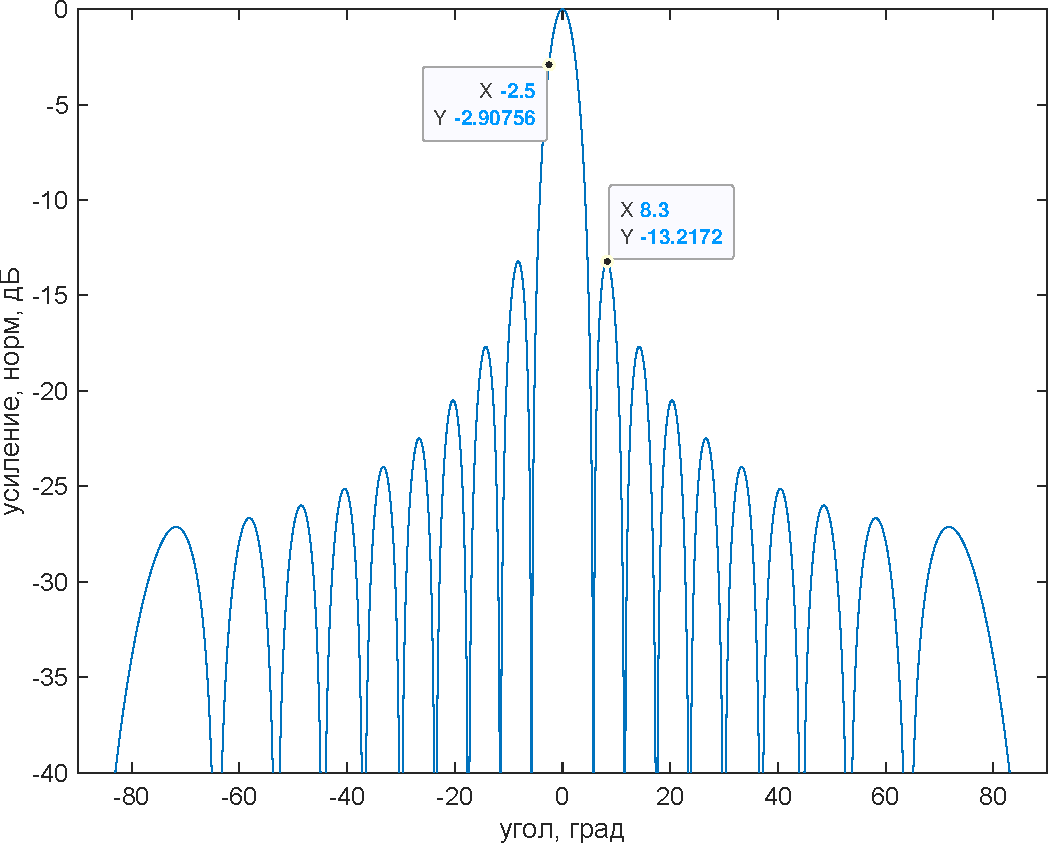
\includegraphics[width=\textwidth]{equally-spaced-distribution-beam-pattern0}
        \caption{}%
        \label{fig:equally-spaced-distribution-beam-pattern0}
    \end{subfigure}
    \hfill
    \begin{subfigure}[b]{0.49\textwidth}
        \centering
        \hspace*{-3ex}
        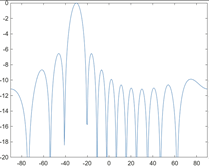
\includegraphics[width=\textwidth]{equally-spaced-distribution-beam-pattern-30}
        \caption{}%
        \label{fig:equally-spaced-distribution-beam-pattern-30}
    \end{subfigure}
    \begin{subfigure}[b]{0.49\textwidth}
        \centering
        \hspace*{-3ex}
        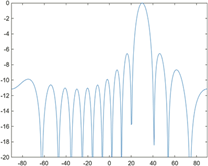
\includegraphics[width=\textwidth]{equally-spaced-distribution-beam-pattern30}
        \caption{}%
        \label{fig:equally-spaced-distribution-beam-pattern30}
    \end{subfigure}
    \caption{%
        ДН при отклонении луча на
        (а) 0
        (б) -30 и
        (в) +30 градусов
    }%
    \label{fig:equally-spaced-distribution}
\end{figure}

Такие антенные решётки применяются и в современных устройствах ввиду простоты их проектирования, 
однако они имеют несколько недостатков: высокий уровень боковых лепестков 
(на Рисунке~\ref{fig:equally-spaced-distribution} видно, что уровень второго лепестка составляет порядка -13 дБ от основного) 
и высокая стоимость из-за большого количества элементов, которое необходимо для поддержания требуемой
ширины основного лепестка при расстоянии между элементами $d \leq \lambda/2$. 
Увеличение же межэлементного расстояния приводит к появлению дифракционных 
лепестков (ложных целей), пример такого явления можно увидеть на Рисунке \ref{fig:equally-spaced-distribution-granting-lobes}.

\begin{figure}[!ht]
    \centering
    \hspace*{-3ex}
    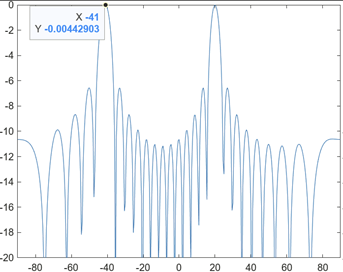
\includegraphics[width=0.8\textwidth,height=0.35\textheight,keepaspectratio]{equally-spaced-distribution-granting-lobes}
    \caption{ДН при межэлементном расстоянии $d > \lambda/2$,
        направленность на~20~градусов,
        дифракционный лепесток~на~-44,5~градусов}%
    \label{fig:equally-spaced-distribution-granting-lobes}
\end{figure}

Потому такие решётки применяются в системах, где отсутствие множественной направленности менее критично, 
чем увеличение размера/веса итогового устройства, например, в системах межспутниковой связи. 
Кроме того, важную роль играет простота изготовления и наладки таких ФАР.

В системах, где параметры направленности являются критичными, а также в тех случаях когда 
есть возможность применять более сложные подходы, используются решётки, разработанные с помощью методов, 
которые будут описаны в следующих разделах данной работы. 

